\newpage
\section{Narzędzia}
\label{cha:Narzędzia}

\subsection{Narzędzia wspomagające zarządzanie projektem}

\subsubsection{GIT}
\label{sub:GIT}
Rozproszony system kontroli wersji. System ten pozwola na bezproblemową synchronizacje pracy między stacjami roboczymi. Dzięki temu, że jest on rozproszony nie jest konieczne wyznaczanie głównego serwera, przez który synchronizowany jest kod źródłowy, a każdy z klientów może pełnić rolę serwera do którego wysyłane są zmiany plików objętych systemem kontroli wersji.

Przy realizacji pracy dyplomowej GIT pomógł rozwiązywać konflikty w treści kodu źródłowego, ciągłe nadpisywanie treści plików powstałe w wyniku pracy kilku osób. Do przechowania kodu źródłowego na serwerze zdalnym wykorzystana została darmowa powierzchnia serwisów GitHub oraz Bitbucket. Na Githubie umieszczone zostały aplikacje stworzone w ramach pracy dyplomowej oraz książka napisana w LaTex.


\subsubsection{Asana}
\label{sub:Asana}

Z racji na sposobność pracy w zespole nad pracą dyplomową niezbędne było narzędzie wspomagające komunikację oraz kontrolę wykonywania zadań. Asana to system zarządzania projektem umożliwiający rozdzielanie zadań pomiędzy członków zespołu przypisanych do projektu, śledzenie postępów prac, ustalania przypomnień oraz terminów. System wspomaga komunikację, dzieli obszary zainteresowań na podprojekty, umożliwia oznaczenie zagadnień słowami kluczowymi oraz udostępnia wyszukiwarkę. Narzędzie dostępne w modelu SaaS (ang. Software as a Service) dostępne przez przeglądarkę internetową bez konieczności instalacji oprogramowania.

W projekcie narzędzie wykorzystane zostało do monitorowania postępów prac oraz tworzenie bazy wiedzy.

\subsection{Narzędzia programistyczne}

\subsubsection{Vim}
\label{sub:Vim}
Prawdopodobnie najpopularniejszy konsolowy edytor tekstu. Vim jest klonem edytora vi, z wieloma nowymi funkcjami. Przede wszystkim jest to modalny edytor tesktu tzn. że posiada więcej niż jeden tryb pracy (INPUT, COMMAND, VISUAL). Dzięki swojej prostocie, szybkości, oraz mnogości wtyczek ten konsolowy edytor jest wciąż bardzo popularny i używany w zastępstwie wielu zintegrowanych środowisk programistycznych jak np. Eclipse czy VisualStudio.  

\subsection{Wykorzystana technologia w pilotach}

\subsubsection{jQuery Mobile}
\label{subsub:tool-jquery-mobile}

Brak respektowania standardów (podsekcja \ref{subsec:w3c-touch-events-implementations}) stwarza problemy związane z obsługą gestów na urządzeniach mobilnych. Aby zapewnić poprawne funkcjonowanie należy śledzić zmiany wprowadzane w implementacjach przeglądarek przez producentów oraz ewentualne zmiany w standardach. W projekcie wykorzystana została biblioteka \emph{jQuery Mobile} posiadająca dużą społeczność\footnote{Ponad 10 tyś poprawek, 36 wersji, 204 osób wnoszących wkład w rozwój biblioteki [Stan na 22 grudnia 2013]}. Wśród wpieranych przeglądarek znajdują się wymienione jako niewspierające standardu z podsekcji ~\ref{subsec:w3c-touch-events-implementations}.

Biblioteka wykorzystywana w zakresie poruszania punktów dotyków definiuje \emph{wirtualną mysz} (oznaczoną \lstinline{vmouse}) jako abstrakcję na standardową mysz lub dotyk na urządzeniu mobilnym. Zdarzenia obsługujące wirtualną mysz będą wyzwalane dla myszy komputerowej oraz dla panelu dotykowego.

Zdarzenie \lstinline{vmousemove} symuluje zdarzenia \lstinline{onmousemove} oraz \lstinline{touchmove}. Przykład użycia:

\lstset{language=JavaScript}
\begin{lstlisting}
$(document).on('vmousemove', function(e) {
	// Zapobieganie dalszej propagacji zdarzenia
	// po przechwyceniu, strona nie bedzie przewijana.
	e.preventDefault();
	
	// Pobieranie pozycji kursora z obiektu zdarzenia.
	var x = e.pageX
	var y = e.pageY
	
	console.log(x, y) // wypisz dane na konsoli
})
\end{lstlisting}

\subsubsection{Użycie biblioteki basket.js}
\label{subsub:tools-basketjs}

W związku z dywagacją dotyczącą szybkości działania Web Storage (podsekcja \ref{subsub:webstorage-performance}), wszystkie skrypty JavaScript pilota są umieszczone z lokalnej pamięci przeglądarki internetowej Web Storage na telefonie komórkowym. W tym celu opracowana została biblioteka \emph{basket.js} oferująca asynchroniczne ładowanie kodu JavaScript z rozwiązaniem zależności między plikami oraz rozgrywaniem wyścigów\footnote{W asynchronicznym modelu programowania kolejne kawałki kodu nie wykonują się sekwencyjnie, co może doprowadzić do błędów wynikających z zależności między nimi}. basket.js jako interfejs dla programisty używa wzorca projektowego \emph{Promise}.

Dla ułatwienia zarządzania kodem wykonującym się asynchronicznie stosuje się najczęściej trzy wzorce projektowe:

\begin{description}
  \item[Callback] \hfill \\
  Polega na zarejestrowaniu funkcji, do której przechodzi się zaraz po wykonaniu asynchronicznej operacji. Przykład:
  \lstset{language=Octave}
  \begin{lstlisting}
  database.query("SELECT * FROM table;", function(data), {
  	console.log(data) // wiersze do wypisania
  })
  \end{lstlisting}
  \lstinline{function(data)} to sygnatura anonimowej\footnote{Anonimowej - nie posiadającej identyfikatora, w konsekwencji nie można jej ponownie użyć.} funkcji. Zamiast sygnatury może zostać podany identyfikator wcześniej zadeklarowanej funkcji. Minusem tego rozwiązania jest fakt, że istnieje tylko jedna funkcja, która reaguje na zakończenie operacji, co w niektórych przypadkach może być utrudniające. Drugim minusem tego rozwiązania jest to, że zarówno w przypadku błędu, jak i powodzenia, wykonywana jest ta sama funkcja.
  \item[Events] \hfill \\
  W odpowiedzi na możliwość reagowania tylko jedną funkcją na zakończenie operacji przychodzi wzorzec projektowy \emph{Events} (ang. zdarzenia), który domyślnie implementuje funkcję, która w pętli iteracyjnie wykonuje wszystkie funkcje zarejestrowane jako callback. Innymi słowy istnieje wiele funkcji callback, które reagują na dane zdarzenie, na przykład:\\

  

  Wzorzec projektowy nie rozwiązuje natomiast problemu, iż w przypadku powodzenia lub niepowodzenia operacji, wykonuje się ten sam zestaw funkcji callback. Z wykonania wielu funkcji callback w systemach, gdzie mogą one zostać równolegle, wzorzec projektowy posiada minus wynikający z synchronizacji funkcji.
  \lstset{language=Octave}
  \begin{lstlisting}
  var funckja1 = function() {
  	console.log('zaszlo zdarzenie klikniecia')
  }
  element.on('click', funkcja1)
  element.on('click', function() {
  	console.log('zaszlo zdarzenie klikniecia')
  })
  \end{lstlisting}
  \item[Promise] \hfill \\
  Jest to wzorzec projektowy deklarujący strukturę funkcji reprezentującą zdarzenie, które zajdzie w przyszłości. Pozwala to na wykonywanie funkcji zarówno jak Events, jak i Callback, bowiem obiekty mogą być łączone w synchroniczny łańcuch.
\end{description}

Przykład użycia biblioteki basket.js jako wzorca projektowego Promise:

\lstset{language=JavaScript}
\begin{lstlisting}
basket
    .require(
		{ url: 'assets/js/jquery-1.10.2.min.js' },
		{ url: 'assets/js/socket.io.js' }
	)
    .then(function() {
        basket.require({ url: 'assets/js/jquery.mobile-1.3.2.min.js' });
    })
	.then(function() {
        basket.require({ url: 'app.js' });
    })
	.then(function() {
	 	// ...
	})
});
\end{lstlisting}

Funkcja \lstinline{require} na rzecz obiektu \lstinline{basket} zwraca obiekt Promise, który uruchamia równolegle trzy funkcje callback. Funkcje callback również mogą zwracać obiekty Promise tworząc synchroniczny łańcuch.

\subsection{Wykorzystana technologia w części serwerowej}
\label{sub:tool-server-technology}

Część serwerowa infrastruktury została napisana w środowisku \emph{Node.js}, stworzonego przez Ryana Dahla w 2009 roku. Node.js używa składni skryptowego\footnote{Kod języków skryptowych wykonywany jest wewnątrz jakiejś aplikacji/środowiska w odróżnieniu od programów napisanych w językach nieskryptowych, które kompilują się i stanowią aplikację} języka JavaScript znanego z tworzenia dynamicznych elementów stron internetowych. Kod JavaScript, choć wykonuje się w ramach przeglądarki internetowej, w Node.js uruchamiany jest po stronie serwera. Technologia umożliwia dużą przepustowość zapewniając nieblokujące operacje wejścia/wyjścia (ang. \emph{non-blocking I/O}) i pętli zdarzeń w pojedynczym wątku \emph{single-threaded event loop}. Podejście to nazywa się programowaniem asynchronicznym (opisanym w podsekcji \ref{subsub:asyncprogramming}).

Wybór platformy obsługującej programowanie asynchroniczne jest jednoznaczny ze względu na specyfikę aplikacji. Większość z nich to oczekiwanie na dane z sieci (ang. \emph{network I/O}). Jeżeli program byłby napisany w modelu synchronicznym, procesor przeznaczałby większość czasu na oczekiwanie na dane z sieci zawieszając (ang. \emph{idle}) jego pracę na funkcjach wejścia/wyjścia. Tymczasem, aby zwiększyć możliwości (uruchomienie tysięcy operacji I/O jednocześnie) korzysta się z asynchronicznego, nieblokującego podejścia pisania aplikacji za pomocą pętli zdarzeń uruchomionej w pojedynczym wątku. Podejście jest odpowiednie do czasu, gdy program nie wykonuje złożonych czasowo operacji, które to mogłyby zawiesić działanie pętli komunikatów uruchomionej w pojedynczym wątku. Większość operacji w stworzonej aplikacji to przekazywanie struktur danych i praca w sieci.

\subsubsection{Synchroniczny i imperatywny model programowania}

W porównaniu do programowania asynchronicznego przedstawione krótko zostanie programowanie imperatywne, będące paradygmatem programowania\cite{programming-paradigms} które opisuje kod programu jako sekwencyjnie wykonywany ciąg instrukcji zmieniający stan programu (rejestrów, pamięci). Takie wyobrażenie przepływu programu jest de facto tożsame z fizyczną realizacją kodu maszynowego na komputerze. W tym modelu przebieg programu możemy zdefiniować jako ciąg następujących po sobie instrukcji\ref{fig:syncprogramming-flow}, dzięki czemu jego przebieg jest przewidywalny, bowiem wykonując bieżącą instrukcję można założyć, ze poprzednia się zakończyła powodzeniem, a jej wyniki są dostępne do użycia. Implikuje to, że wykonywanie każdej operacji jest blokujące\ref{fig:syncprogramming-waiting}. Rozwiązaniem tego problemu jest uruchamianie przebiegu programu w wątkach\ref{fig:syncprogramming-threads} mogących komunikowanie się między sobą lub uruchomienie programu jako nowy proces w systemie operacyjnym\footnote{Te zabiegi powodują narzut czasowy związany z przełączaniem kontekstu pracy procesora w postaci odłożeniem stanu rejestrów, mapy pamięci, rejestrów stosu, FPU itd.}.

\begin{figure}[ht]
\centering
\begin{minipage}[b]{0.45\linewidth}
  \label{fig:syncprogramming-flow}
  \caption[Programowanie synchroniczne - przebieg instrukcji programu w czasie]{Programowanie synchroniczne - przebieg instrukcji programu w czasie}
  \centering
    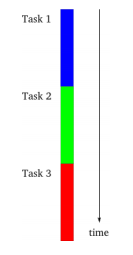
\includegraphics[scale=0.5]{syncprogramming-flow.png}
\end{minipage}

\begin{minipage}[b]{0.45\linewidth}
\label{fig:syncprogramming-threads}
  \caption[Programowanie synchroniczne - wątki]{Programowanie synchroniczne - wątki}
  \centering
    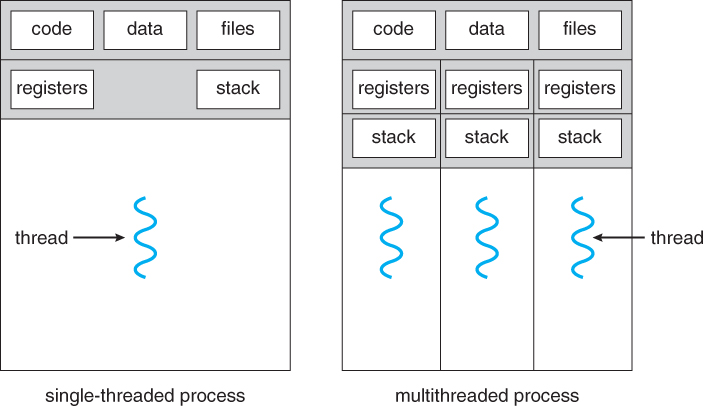
\includegraphics[scale=0.5]{syncprogramming-threads.jpg}
\end{minipage}

\begin{minipage}[b]{0.45\linewidth}
\label{fig:syncprogramming-waiting}
  \caption[Programowanie synchroniczne - operacje blokujące]{Programowanie synchroniczne - operacje blokujące}
  \centering
    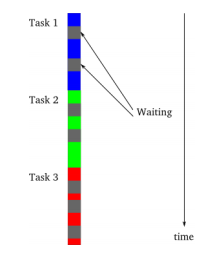
\includegraphics[scale=0.5]{syncprogramming-waiting.png}
\end{minipage}
\end{figure}

\subsubsection{Asynchroniczny model programowania}
\label{subsub:asyncprogramming}

Asynchroniczny model programowania oparty jest na programie uruchomionym w jednym wątku. Znany jest z frameworków graficznych interfejsów użytkownika GUI (na przykład WinApi). W uproszczeniu, budowa programu to nieskończona pętla oraz kolejka operacji odłożona na stos. Z każdym przebiegiem pętla sprawdza w kolejce operacji, czy możliwe są do wykonania jakieś operacje, jeżeli tak, uruchamiane są procedury obsługi (ang. \emph{handlers} lub \emph{callbacks}). Umożliwia to realizację wielu operacji, które oczekują na wyniki bez blokowania pracy całego programu.

\begin{figure}[H]
  \caption[Event loop w asynchronicznym modelu programowania]{Event loop w asynchronicznym modelu programowania}
  \centering
    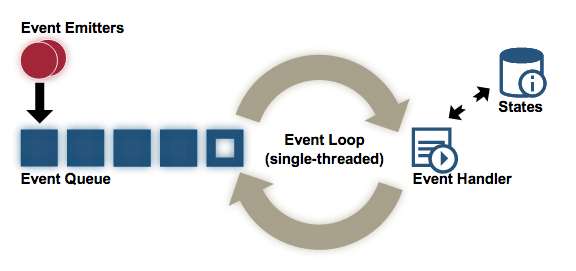
\includegraphics[width=\linewidth]{asyncprogramming-loop.png}
\end{figure}

Realizacja niskopoziomowa to użycie funkcji \lstinline{select()} (zarówno systemów POSIX jak i Windows), deskryptorów \lstinline{/dev/poll}, kqueue, poll i epool. Warta rozpoznania jest biblioteka \emph{libevent}\footnote{\url{http://libevent.org/}}, która zakłada abstrakcję na użyte mechanizmy z punktu widzenia programisty\cite{programming-async-sockets}.

Funkcja \lstinline{select()} przyjmuje za parametry deskryptory oraz maksymalny czas upływu. Zwraca wartość jeżeli a) upłynie zdefiniowany czas lub b) gdy w deskryptorze (reprezentującym plik, urządzenie, gniazdo sieciowe lub strumień danych) zajdą zmiany - będzie dostępny do zapisu lub są dostępne dane do odczytu:

\lstset{language=C}
\begin{lstlisting}
#include <sys/time.h>
#include <sys/types.h>
#include <unistd.h>

int select(int numfds, fd_set *readfds, fd_set *writefds,
           fd_set *exceptfds, struct timeval *timeout);
\end{lstlisting}

W przeciwieństwie do synchronicznego modelu w programowaniu imperatywnym, model asynchroniczny wypada korzystniej, gdy\cite{programming-async}:

\begin{enumerate}
  \item Zadania są zupełnie niezależne od siebie, nie jest konieczna komunikacja między nimi, ani oczekiwanie na rezultaty.
  \item Zadania wykonują wiele operacji wejścia/wyjścia (I/O) powodujących, że program synchroniczny zostaje zawieszony do momentu otrzymania rezultatu, wtenczas może wykonywać inne zadania.
\end{enumerate}

Zatem program napisany asynchronicznie blokuje swoje działanie tylko wtedy, gdy nie ma zadań do wykonania i nie jest możliwy dalszy postęp przebiegu programu (dlatego jest nazywany nieblokującym). Przy wykonaniu wielu blokujących zadań program napisany asynchronicznie może być znacznie szybszy spędzając mniej czasu na czekaniu na wyniki, a wykonując wiele pojedynczych zadań podczas przebiegu pętli.

\subsubsection{Zasada działania Node.js}
\label{sub:tool-server-nodejs}

Node.js jest środowiskiem używającym składni skryptowego języka JavaScript\footnote{Po kliku nieudanych próbach implementacji w C, Lua,  Haskell, twórca Node.js Ryan Dahl, po pojawieniu się Google JavaScript Engine V8 zdecydował się na jego użycie}, udostępniającym mechanizmy programowania asynchronicznego opartego o wywołania funkcji \emph{callbacks}. Node.js działa w pojedynczym wątku opartym o pętlę zdarzeń obsługiwanych przez procedury obsługi (callbacks). Środowisko oparte jest na projekcie opensource \emph{V8 Javascript Engine} wydanym przez Google, który (w odróżnieniu od innych) kompiluje JavaScript do kodu maszynowego\footnote{Obsługiwane platformy: IA-32, x86-64, ARM oraz MIPS ISAs} przed jego wykonaniem.

\begin{figure}[H]
  \caption[Model działania Node.js]{Model działania Node.js na przykładzie serwera HTTP}
  \centering
    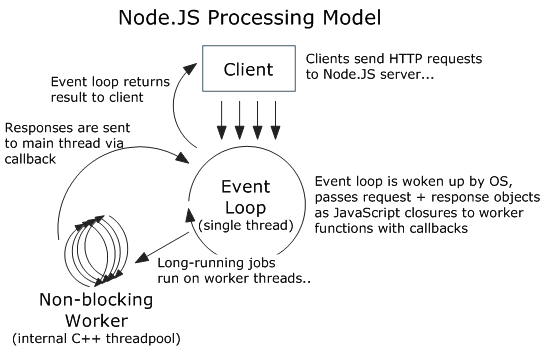
\includegraphics[scale=0.75]{nodejs-flow.png}
\end{figure}

\subsubsection{Socket.io}
\label{subsub:socketio}

Socket.io to biblioteka Node.js, która zapewnia komunikację dwukierunkową między przeglądarka użytkownika, a serwerem. Co ważne, sposób wykorzystania biblioteki zarówno po stornie serwera, jak i klienta jest taki sam. Komunikacja zapewniana jest przez wspierane sposoby opisane w podrozdziale \ref{sub:communication-methods})\footnote{http://socket.io/\#browser-support}:

\begin{enumerate}
  \item WebSocket
  \item Adobe® Flash® Socket
  \item AJAX long polling
  \item AJAX multipart streaming
  \item Forever Iframe
  \item JSONP Polling
\end{enumerate}

Przykładowy node.js kod po stronie serwera:

\lstinputlisting[language=JavaScript]{assets/src/socketio-example-server.js}

Powyższy kod uruchamia serwer nasłuchujący na porcie 8081, i przyjmuje zgłoszenia. Gdy klient się podłączy, dodawany jest callback na rzecz obiektu klienta \lstinline{socket} na wiadomość nazwaną \emph{the message from client}, który jest wykonywany, gdy wiadomość o takim identyfikatorze nadejdzie, za pomocą konstrukcji \lstinline{socket.on('the_message_from_client', function(data)}. Wysyłanie wiadomości podłączonemu klientowi odbywa się poprzez wywołanie metody emit na rzecz obiektu klienta socket \lstinline{socket.emit('the_message_from_server', function(data)} , która przyjmuje argument jako nazwę wiadomości \emph{the message from server} oraz drugi w postaci obiektu JavaScript, który zostanie zserializowany do formatu JSON i wysłany jako tekst, gdzie po stornie klienta zostanie zdeserializowany i zinterpretowany również jako obiekt JavaScript.

Przykładowy kod po stornie klienta:

\lstinputlisting[language=JavaScript]{assets/src/socketio-example-client.js}

Kod jest bliźniaczo podobny do kodu uruchamianego na serwerze. Klient ustanawia połączenie do adresu podanego jako argument funkcji \lstinline{connect}. Domyślnie używany jest protokół WebSocket ws://, można skorzystać z szyfrowanego protokołu wss://\footnote{analogiczny http:// do https://} wskazując go przed nazwę hosta. Istnieje możliwość skonfigurowania połączenia, np wskazać, czy ma zostać podjęta próba ponownego połączenia przy jego utracie.


\subsection{Wykorzystane technologie i narzędzia w serwerze zarządzającym infrastrukturą}

\subsubsection{SBT}

SBT (ang. \emph{Simple Build Tool}) to narzędzie służące do budowania projektów, rozwiązywanie zależności, podobne jest bardzo do bardziej znanych tego typu narzędzi jak Maven, czy Ant. Natomiast w przeciwieństwie do tych narzędzi cała konfiguracja odbywa się w jednym pliku i do tego napisanym w języku Scala. Nie jest również niezbędna dodatkowa integracja środowiska programistycznego. By dodać nową zależność do projektu, należy otworzyć plik \lstinline|Build.sbt| i dodać zależność według następującego schematu:

\begin{lstlisting}
//identyfikator grupy    %%     identyfikator artefaktu  %   wersja
"com.decodified"         %%     "scala-ssh"              %   "0.6.4"
\end{lstlisting}

Standardowo SBT korzysta tylko z publicznych standardowych repozytoriów, by dodać nowe (mogą to być repozytoria Maven czy Ivy), należy w tym samym pliku dodać je według następującego przykładu:

\begin{lstlisting}
resolvers += "spray repo" at "http://repo.spray.io"
\end{lstlisting}

\subsubsection{Akcje}

W kontrolerach (które w scali są obiektami) definiowane są metody, każda z metod odpowiada za konkretną akcje, odpowiadając na żądanie użytkownika. Proszę przyjrzeć się następującemu kontrolerowi:

\begin{lstlisting}
object Application extends Controller {
  def index = Action {
    Ok("It works!")
  }
}
\end{lstlisting}

Obiekt \lstinline{Application} dziedziczy po cesze \lstinline{Controller}, która głównie zapewnia szereg metod pomocniczych do zdefiniowania akcji. Metoda \lstinline{index} jest definiowana przez funkcję \lstinline{Action} (reprezentowana w Javie jako obiekt), która jako argument przyjmuje obiekt \lstinline{Request}, a zwraca obiekt \lstinline{Response}. 

\par

Tak zdefiniowana akcja definiuje blok kodu w sposób synchroniczny zwracający wynik, jednak aplikacje internetowe coraz częściej zorientowane są wokół usług internetowych (ang. \emph{Web Services}), które w sporej większości nie mają WSLA \footnote{ang. \emph{Web Service Legal Agreement} umowa utrzymania jakości usług. Pozwala autorom na wyszczególnienie wymagań co do usługi, oraz akcji, które powinny zostać podjęte podczas gdy te nie zostaną spełnione}. Tutaj z pomocą przychodzi framework Play z technologią rozwiązującą tego typu problemy.

Framework Play w zamierzeniu działa na bardzo małym zbiorze wątków, dlatego też podczas gdy dana akcja nie może odpowiedzieć natychmiastowo np. z powodu usługi internetowej czy długiego zapytania do bazy danych, wątek obsługujący daną akcje nie może zostać zablokowany. 

\begin{description}	
	\item[Future] \hfill \\
		Za pomocą zmiennej o tym typie, można uzyskać wartość, kiedy tylko zostanie obliczona, pobrana.
	\item[Promise] \hfill \\
		Typ Promise działa w przeciwną stronę tzn. jeżeli \lstinline{Future} jest typem konsumenta, tak \lstinline{Promise} jest typem charakterystycznym dla producenta. Za każdym razem gdy programista chcę obliczyć lub pobrać jakieś dane tworzy obiekt \lstinline{Promise}, który jest kontenerem na nowe dane. Z obiektu \lstinline{Promise} otrzymuje się obiekt typu \lstinline{Future}.
\end{description}

\begin{lstlisting}
def index = Action.async {
  val foo: Future[Foo] = getFoo()
  foo.map(f => Ok(f))
}
\end{lstlisting}

\par

W linii pierwszej powyższego listingu definiowana jest nie tyle funkcja Action co Action.async stworzone przez wzorzec budowniczego, który to właśnie powoduje, że wątek obsługujący tą akcje jest zwalniany, i system wraca do wykonania tej metody podczas gdy zmienna foo zostanie pobrana/obliczona.

\par
Interesująca funkcjonalność jest zaprezentowana w linii trzeciej. Funkcja \lstinline{map} wywołana na obiekcie \lstinline{Future}, zwraca rezultat podczas gdy obiekt \lstinline{foo} zostanie uzupełniony. Mechanizm ten jest o tyle interesujący, że w innych językach programowania jest to wykonywane za pomocą funkcji \lstinline{onSuccess}. Takie rozwiązanie w przykładzie, który został przedstawiony byłoby jak najbardziej dopuszczalne natomiast rozważając inny bardziej skomplikowany przypadek:

\begin{lstlisting}
val rateQuote = future {
  connection.getCurrentValue(USD)
}
rateQuote onSuccess { case quote =>
  val purchase = future {
    if (isProfitable(quote)) connection.buy(amount, quote)
    else throw new Exception("not profitable")
  }
  
  purchase onSuccess {
    case _ => println("Purchased " + amount + " USD")
  }
}
\end{lstlisting}

Używając metody \lstinline{onSuccess} zagnieżdżamy wykonanie kolejnej operacji. Przedstawione rozwiązanie nie jest najlepsze z dwóch powodów:
\begin{itemize}
	\item Każde kolejne zagnieżdżenie następnej operacji powoduje, że kod staję się nieczytelny (ang. \emph{Callback Hell})
	\item Kod wywołujący zagnieżdżoną operację jest zagnieżdżony co uniemożliwia wywołanie ponownie tego samego kodu z innego miejsca programu.
\end{itemize}
